\section*{\hfill{}УСЛОВИЕ\hfill{}}
В информационный центр приходят клиенты через интервал времени 10 $\pm$ 2 минуты. Если все три имеющихся оператора заняты, клиенту отказывают в обслуживании. Операторы имеют разную производительность и могут обеспечивать обслуживание среднего запроса пользователя за 20 $\pm$ 5; 40 $\pm$ 10; 40 $\pm$ 20. Клиенты стремятся занять свободного оператора с максимальной производительностью. Полученные запросы сдаются в накопитель. Откуда выбираются на обработку. На первый компьютер запросы от 1 и 2-ого операторов, на второй – запросы от 3-его. Время обработки запросов первым и 2-м компьютером равны соответственно 15 и 30 мин. Промоделировать процесс обработки 300 запросов. Определить вероятность отказа.

\section*{\hspace{1.25cm}1\quad{}Теоретическая часть}
На рисунке\ref{img:concept} изображена структурная схема рассматриваемой концептуальной модели.
\begin{figure}[H]
    \centering
    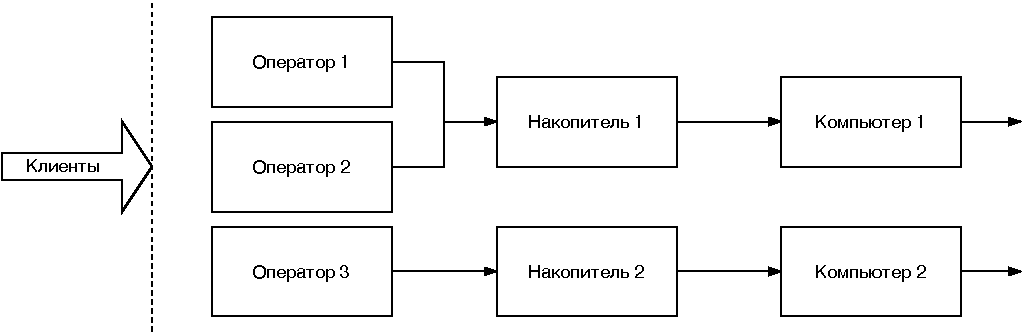
\includegraphics[width=0.8\textwidth]{pdf/concept.pdf}
    \caption{Структурная схема}
    \label{img:concept}
\end{figure}

\section*{\hspace{1.25cm}2\quad{}Практическая часть}

\begin{lstlisting}[caption={Текст программы},label={lst:model}]
GENERATE	10,2,0,300 ; Ввод транзактов в модель:
	                   ; со средним временным интервалом появления 10;
		               ; разбросом 2;
		               ; временем появления первого транзакта 0;
		               ; общим числом генерируемых транзактов 300.


OPERATOR1    GATE NU 	 OPER1,OPERATOR2 ; Если первый оператор занят,
                                         ; переход ко второму
	SEIZE	 OPER1       ; Занять первого оператора
	ADVANCE	 20,5        ; Задержка транзакта на 20 с разбросом 5
	RELEASE	 OPER1       ; Освободить первого оператора
	TRANSFER ,COMPUTER1  ; Переход к первому компьютеру

OPERATOR2	 GATE NU	 OPER2,OPERATOR3 ; Если второй оператор занят,
                                         ; переход к третьему
	SEIZE	 OPER2       ; Занять второго оператора
	ADVANCE	 40,10       ; Задержка транзакта на 40 с разбросом 10
	RELEASE	 OPER2       ; Освободить второго оператора
	TRANSFER ,COMPUTER1  ; Переход к первому компьютеру

OPERATOR3	 GATE NU	 OPER3,REJECT    ; Если третий оператор занят,
                                         ; переход к отказу на заявку
	SEIZE	 OPER3       ; Занять третьего оператора
	ADVANCE	 40,20       ; Задержка транзакта на 40 с разбросом 20
	RELEASE	 OPER3       ; Освободить третьего оператора
	TRANSFER ,COMPUTER2  ; Переход ко второму компьютеру

COMPUTER1    QUEUE	QUEUE1   ; Помещение транзакта в конец очереди QUEUE1
	SEIZE	 COMP1    ; Занять первый компьютер
	DEPART	 QUEUE1   ; Удаление транзакта из очереди QUEUE1
	ADVANCE	 15       ; Задержка транзакта на 15		 
	RELEASE	 COMP1    ; Освободить первый компьютер
	TRANSFER ,SUCCESS ; Переход к завершению успешного выполнения

COMPUTER2	 QUEUE	QUEUE2   ; Помещение транзакта в конец очереди QUEUE2
	SEIZE 	 COMP2    ; Занять второй компьютер
	DEPART	 QUEUE2   ; Удаление транзакта из очереди QUEUE2
	ADVANCE	 30       ; Задержка транзакта на 30		
	RELEASE	 COMP2    ; Освободить второй компьютер
	TRANSFER ,SUCCESS ; Переход к завершению успешного выполнения

SUCCESS	TRANSFER 	,FINAL   ; Переход к завершению
REJECT	TRANSFER	,FINAL   ; Переход к завершению


FINAL	SAVEVALUE REJECT_QTY,N$REJECT  ; Количество отказанных заявок
        ; Вероятность отказа
    	SAVEVALUE PROBABILITY,((N$REJECT)/(N$SUCCESS + N$REJECT))
    	TERMINATE	1
    	START 300
\end{lstlisting}

На рисунке~\ref{img:results} представлены результаты выполнения программы на GPSS.
\begin{figure}[H]
    \centering
    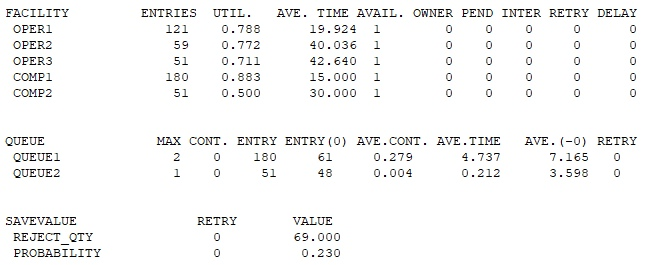
\includegraphics[width=0.8\textwidth]{images/scr01.jpg}
    \caption{Результаты}
    \label{img:results}
\end{figure}

\section*{\hfill{}ВЫВОД\hfill{}}
В настоящей лабораторной работе была промоделирована информационная система, в которую поступают клиенты. Эта система состоит нескольких блоков, а именно: генератор заявок, три оператора, два накопителя и два компьютера. Выходными данными являются вероятность отказа и количество клиентов, отказ получивших.
